\documentclass[12pt,a4paper]{scrreprt}

\usepackage{graphicx}
\usepackage{a4}
\usepackage[ngerman]{babel}
\usepackage[utf8]{inputenc}
\usepackage{hyperref}
\usepackage[nottoc,notindex,notlot]{tocbibind}
\usepackage{nameref}
\usepackage{subcaption}
\usepackage{listings}
\usepackage{color}
\usepackage{xcolor}
\usepackage{longtable}
\usepackage{amsmath}

\lstdefinestyle{MyCodeStyle}{
	belowcaptionskip=1\baselineskip,
	breaklines=true,
	frame=single,
	captionpos=b,
	numbers=left,
	xleftmargin=\parindent,,
	showstringspaces=false,
	basicstyle=\footnotesize\ttfamily,
	keywordstyle=\bfseries\color{green!40!black},
	commentstyle=\itshape\color{purple!40!black},
	identifierstyle=\color{blue},
	stringstyle=\color{orange}
}
\lstset{escapechar=@,style=MyCodeStyle}

\newcommand{\includecode}[3]{\lstinputlisting[label=#1,caption=#2,float=ht,aboveskip=0pt,belowskip=0pt]{#3}}
\newcommand{\absatz}{\\[12pt]}

\newcommand{\thema}{Parallelisierter Genetischer Algorithmus für das TSP}
\newcommand{\abgabedatum}{30.08.2016}
\newcommand{\autorTitel}{Timo Bertsch\\Joram Markert\\Fabian Meyer}
\newcommand{\autorAbs}{Timo Bertsch\\ & Joram Markert\\ & Fabian Meyer}
\newcommand{\studiengang}{Master Computer Science}
\newcommand{\prueferA}{Prof. Dr. Lutz Köhler}
\newcommand{\prueferB}{Pascal}

\newcommand{\zusammenfassung}{Lorem ipsum dolor sit amet, consetetur sadipscing elitr, sed diam nonumy eirmod tempor invidunt ut labore et dolore magna aliquyam erat, sed diam voluptua. At vero eos et accusam et justo duo dolores et ea rebum. Stet clita kasd gubergren, no sea takimata sanctus est Lorem ipsum dolor sit amet. Lorem ipsum dolor sit amet, consetetur sadipscing elitr, sed diam nonumy eirmod tempor invidunt ut labore et dolore magna aliquyam erat, sed diam voluptua. At vero eos et accusam et justo duo dolores et ea rebum. Stet clita kasd gubergren, no sea takimata sanctus est Lorem ipsum dolor sit amet.}

\begin{document}

\begin{titlepage}

\vspace*{-3.5cm}

\begin{flushleft}
\hspace*{-1cm} 
\includegraphics[width=3.5cm]{thkoeln-logo}
\end{flushleft}

\vspace{2.5cm}

\begin{center}
	\huge{
		\textbf{\thema} \\[4.5cm]
	}
	\Large{
		\textbf{\autorTitel}} \\[1.5cm]
		\large{
		\textbf{\studiengang} \\[8cm]
	}
	\large{
		\textbf{Gummersbach, \abgabedatum} \\[2.3cm]
	}
\end{center}

\end{titlepage}

\pagenumbering{arabic}

\begin{center}
{\Large \textbf{Abstract}}
\end{center}

\bigskip

\begin{center}
	\begin{tabular}{p{2.8cm}p{10cm}}
		Thema: & \thema \\
		 & \\
		Author: & \autorAbs \\
		 & \\
		Prüfer: & \prueferA  \\[.5ex]
		 &  \prueferB \\
		 & \\
		Datum: & \abgabedatum \\
		 & \\
	\end{tabular}
\end{center}

\bigskip

\noindent
\zusammenfassung
\tableofcontents

\setlength{\parindent}{0pt}

\chapter{Einleitung}
\label{chap:einleitung}

einleitungs blabla

\chapter{Das Travelling Salesman Problem}
\label{chap:tsp}

Was ist das problem / Ziel? Auf kombinatorische explosion eingehen; Quellen suchen und erklörung darauf stützen

\chapter{Der Genetische Algorithmus}
\label{chap:algorithmus}

Im Rahmen dieses Projektes wurde ein genetischer Algorithmus entwickelt, mit dem das TSP gelöst wird. Genetische Algorithmen werden im Allgemeinen zur Lösungsfindung bei komplexen Suchproblemen verwendet, bei denen eine kombinatorische Explosion vorliegt und der Lösungsraum so groß ist, dass eine Lösung mit einer optimalen Brute Force Methode nicht möglich ist.\absatz
Die allgemeine Funktionsweise dieses Algorithmus und die Varianten, die in diesem Projekt eingesetzt wurden, werden in \autoref{sec:funktionsweise} erläutert. Der Basisalgorithmus ist jedoch nicht nebenläufig konzipiert, daher mussten einige Modifikationen vorgenommen werden, um diesen in einem verteilten System einsetzen zu können. Diese Änderungen werden in \autoref{sec:parallelisierung} näher beschrieben.

\section{Funktionsweise}
\label{sec:funktionsweise}

Genetische Algorithmen basieren auf der Idee der natürlichen Auslese und ermitteln durch Selektion, Kombination und Evolution von möglichen Lösungen eine sehr gute bis perfekte Lösung für das gesuchte Problem.\\
Eine Lösung des gegebenen Problems wird als \textit{Individuum} bezeichnet. Im Rahmen des TSP sind Individuen Wege, die die Lösungskriterien des TSP erfüllen (siehe \autoref{chap:tsp}). Die Reihenfolge der Knoten, die bei einem Individuum besucht werden, werden als dessen Eigenschaften oder Gene bezeichnet. Eine Menge von Individuen, auf der der Algorithmus operiert, wird \textit{Population} genannt. Der genetische Algorithmus arbeitet iterativ in sogenannten \textit{Generationen}. Die Individuen einer Population werden schrittweise in sogenannten \textit{Generationen} mit einer \textit{Fitness} bewertet, aussortiert und rekombiniert, um die Qualität der Lösungen zu verbessern. Die Phasen einer Generation werden in \autoref{tbl:phasen-algorithmus} zusammenfassend dargestellt (vgl. \cite{jacobsen12A}).
\pagebreak
\begin{center}
\begin{longtable}{p{3.0cm} p{10cm}}

Phase & Beschreibung \\
\hline \\
\textit{Initialisation} & Generiert die initiale Population und wird nur ein einziges Mal zu Beginn des Algorithmus ausgeführt. Die Population wird mit zufällig generierten Individuen erstellt.\\
 & \\
\textit{Evaluation} &  Die Individuen der aktuellen Generation werden mit einem Fitnesswert bewertet. Dieser Zahlenwert drückt aus wie gut das Individuum bzw. die Lösung des des Problems ist. In Bezug auf das TSP bedeutet eine kürzere Strecke der Lösung eine höhere Fitness des entsprechenden Individuums.\\
 & \\
\textit{Selection} & Aus den Individuen der aktuellen Generation werden diejenigen ausgewählt, die für die Crossover Phase verwendet und die in die nächste Generation übernommen werden. Hierbei ist es von zentraler Bedeutung, dass Individuen mit hoher Fitness mit einer höheren Wahrscheinlichkeit ausgewählt werden als die Individuen mit niedriger Fitness.\\
 & \\
\textit{Crossover} & Aus den ausgewählten Individuen (sog. Eltern) werden duch die Kombination von deren Eigenschaften neue Individuen (sog. Kinder) erzeugt, die in die nächste Generation übernommen werden. In Bezug auf das TSP werden hier Teilwege der Eltern so miteinander, dass die Kinder wieder eine valide Lösung des TSP darstellen.\\
 & \\
\textit{Mutation} & Die Gene der erzeugten Kinder werden per Zufall verändert, um eine Stagnation des Genpools zu verhindern und neue Lösungsmöglichkeiten zu erzeugen. Diese Stagnation kann auftreten, wenn über mehrere Generationen hinweg besonders fitte Individuen die Population dominieren.\\

\caption{Phasen des genetischen Algorithmus}
\label{tbl:phasen-algorithmus}
\end{longtable}
\end{center}

Die Umsetzung dieser Phasen im Rahmen dieses Projekts wird in den folgenden Unterabschnitten anhand des Beispielgraphen in \autoref{fig:algo-sample} detailliert beschrieben.

\begin{figure}[ht]
  	\centering
	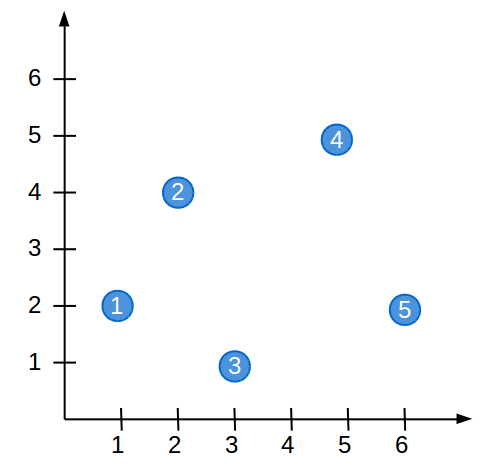
\includegraphics[width=400pt]{images/algo_01_sample.png}
	\caption{Beispielgraph}
	\label{fig:algo-sample}
\end{figure}

Dieses Beispiel zeigt einen Graphen mit fünf Knoten, die jeweils durch die Nummer in ihrer Mitte identifiziert werden können.

\subsection{Initialisation}
\label{subsec:initialisation}

Die \textit{Initialisation} Phase wird nur ein Mal zu Beginn des Algorithmus ausgeführt. In dieser Phase wird die initiale Population generiert, mit der der Algorithmus dann arbeitet. Die Individuen werden hierbei vollständig zufallsgeneriert, wobei jedes Individuum eine valide Lösung des TSP darstellt. Dieser Vorgang wird in \autoref{lst:algo-generierung} dargestellt.

\includecode{lst:algo-generierung}{Generierung eines Individuums}{code/algo_01_generierung.pseudo}

Um ein Individuum zu generieren, wird eine Liste (\textit{nodes}) aller möglichen Knoten für das Individuum, also Knoten aus dem Graphen, erstellt (l. 1). Aus dieser Liste wird dann ein Knoten zufällig ausgewählt (l. 5) und dem Individuum hinzugefügt (l. 6). Danach wird der Knoten aus der Liste der übrigen Knoten entfernt (l. 7) und dieser Prozess wird solange wiederholt bis keine Knoten mehr in \textit{nodes} vorhanden sind (l. 4).\absatz
Mit diesem Verfahren können die Individuen in \autoref{fig:algo-sample-individuals} aus dem Beispielgraphen in \autoref{fig:algo-sample} generiert werden.

\begin{figure}[ht]
  	\centering
	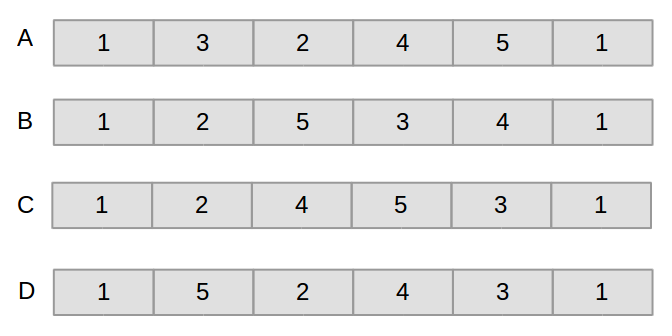
\includegraphics[width=400pt]{images/algo_02_init.png}
	\caption{Beispiel: Zufällig generierte Individuen}
	\label{fig:algo-sample-individuals}
\end{figure}

\subsection{Evaluation}
\label{subsec:evaluation}

In der \textit{Evaluation} Phase werden die Individuen der Population der aktuellen Generation bewertet und damit ihr Fitness Wert errechnet. Jedes Individuum stellt einen Weg durch den Graphen, also eine Liste aufeinander folgender Knoten, dar. Die Fitness errechnet sich aus der Länge dieses Weges. Diese Länge wird durch die Summe des euklidischen Abstands zwischen in der Liste aufeinanderfolgende Knoten beschrieben, wie in der folgenden Gleichung dargestellt wird.

$$
l_{individuum} = \sum_{i=1}^{n} \sqrt{(x_{i+1} - x_i)^2 + (y_{i+1} - y_i)^2}
$$

Dies wird für alle Individuen wiederholt. Hierbei gilt, dass umso länger der Weg ist umso niedriger ist der Fitnesswert eines Individuums. Damit verhält sich die Fitness also \textit{antiproportional} zur Länge des Weges.\\
Aufgrund von Rundungsfehlern bei Gleitkommazahlen reicht ein einfacher Kehrwert der Länge des Weges nicht aus um die Fitness eines Individuums zu berechnen, da der Weg je nach Größe des Graphen entsprechend lang werden kann. Daher wird aus allen Individuen der aktuellen Population dasjenige gesucht, das den längsten Weg $l_{max}$ besitzt. Mit diesem Wert wird nun die Fitness $f_{individuum}$ jedes Individuums auf folgende Weise berechnet.

$$
f_{individuum} = \frac{l_{max}}{l_{individuum}}
$$

\autoref{tbl:algo-sample-fitness} zeigt die Weglänge und die Fitness der Individuen aus \autoref{fig:algo-sample-individuals}.

\begin{center}
\begin{longtable}{p{2.5cm} | p{6.5cm} | p{3.0cm}}
Individuum & $l_{individuum}$ & $f_{individuum}$ \\
\hline & & \\
A & $1 + \sqrt{10} + \sqrt{10} + \sqrt{10} + 5 = 15.49$ & $\frac{19.34}{15.49} = 1.25$ \\
& & \\
B & $\sqrt{5} + \sqrt{20} + \sqrt{10} + \sqrt{20} + 5 = 19.34$ & $\frac{19.34}{19.34} = 1$ \\
& & \\
C & $\sqrt{5} + \sqrt{10} + \sqrt{10} + \sqrt{10} + 1 = 12.72$ & $\frac{19.34}{12.72} = 1.52$ \\
& & \\
D & $5 + \sqrt{20} + \sqrt{10} + \sqrt{20} + 1 = 18.11$ & $\frac{19.34}{18.11} = 1.07$\\

\caption{Beispiel Fitness und Distanz}
\label{tbl:algo-sample-fitness}
\end{longtable}
\end{center}

\subsection{Selection}
\label{subsec:selection}

Während der \textit{Selection} Phase werden die Individuen (Eltern) ausgewählt, aus denen die Individuen für die nächste Generation (Kinder) generiert werden. Die Auswahl geschieht anhand der Fitness der Individuen.Wichtig ist hierbei auch, dass ein einzelnes Individuum mehrfach ausgewählt werden kann.\\
In diesem Projekt wurde zur Auswahl der Eltern das \textit{Roulette-Wheel-Verfahren} verwendet. Hierbei werden die Individuen durch eine Zufallszahl ausgewählt, doch haben besonders fitte Individuen eine besonders hohe Chance ausgewählt zu werden. Hierbei wird die Fitness der Individuen auf das Intervall [0;1] normiert. Daraufhin wird eine Auswahlintervall für jedes Individuum berechnet, indem die Liste der Individuen angefangen beim fittesten Individuum durchlaufen wird und die Fitness aller vorangegangenen Individuen aufsummiert wird. Der sich daraus ergebende Wert ist die untere Grenze $g_{x unten}$ des Auswahlintervalls des Individuums $x$. Die obere Grenze $g_{x oben}$ wird durch die Summe aus unterer Grenze und der Fitness des aktuellen Individuums gebildet (vgl. \cite{rongqu14}). Die folgenden Gleichungen beschreiben den Rechenweg nochmals.

$$
g_{x unten} = \sum_{i=1}^{i<x} f_i
$$
$$
g_{x oben} = g_{x unten} + f_x
$$

\autoref{fig:algo-sample-interval} zeigt die Auswahlintervalle der Individuen aus \autoref{fig:algo-sample-individuals}.

\begin{figure}[ht]
  	\centering
	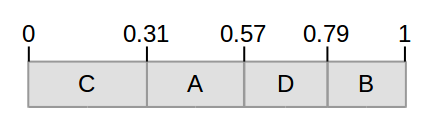
\includegraphics[width=300pt]{images/algo_03_interval.png}
	\caption{Beispiel: Auswahlintervalle der Individuen}
	\label{fig:algo-sample-interval}
\end{figure}

Nun wird eine Zufallszahl im Intervall [0;1] gewürfelt und es wird dasjenige Individuum zum Elternteil erwählt in dessen Intervall die Zufallszahl fällt. Dabei werden immer paare von zwei Eltern gebildet, aus denen ein neues Individuum generiert wird. Dies wird solange wiederholt bis genügend Individuen ausgewählt wurden um die aktuelle Population vollständig zu ersetzen.\absatz
Zusätzlich zur Auswahl der Individuen verwendet der Algorithmus außerdem eine \textit{Elitism} Mechanik, durch die die besten Individuen der aktuellen Generation in die nächste Generation übernommen werden. So wird verhindert, dass bereits gefundene sehr gute Lösungen wieder verworfen werden. Alle anderen Individuen der aktuellen Generation werden jedoch durch neue Individuen, die Kinder, ersetzt.

\subsection{Crossover}
\label{subsec:crossover}

In der \textit{Crossover} Phase werden die aus der \textit{Selection} Phase aus"-ge"-wähl"-ten Eltern kombiniert, um neue Individuen für die nächste Generation zu generieren.\\
Hierbei wird ein zusammenhängender Teilweg des El"-tern"-indi"-vid"-uums A aus zu"-fä"-llig ausgewählt und genau so in das Kind E übernommen. Um die restlichen Knoten des Kindes zu füllen werden der Reihe nach Knoten aus Elternindividuum B Knoten entnommen, falls diese in dem Kind noch nicht vorhanden sind, und in das Kind eingefügt (vgl. \cite{jacobsen12B}). In \autoref{fig:algo-sample-crossover} wird dieser Prozess nochmal verdeutlicht.
\pagebreak

\begin{figure}[ht]
	\centering
	\begin{subfigure}[t]{400pt}
    	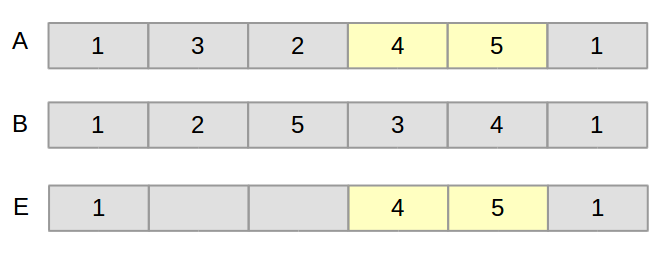
\includegraphics[width=400pt]{images/algo_04_crossover_1.png}
        \caption{}
        \label{fig:algo-sample-crossover1}
    \end{subfigure}

    \begin{subfigure}[t]{400pt}
    	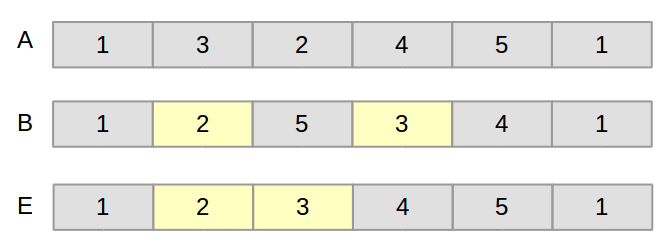
\includegraphics[width=400pt]{images/algo_04_crossover_2.png}
        \caption{}
        \label{fig:algo-sample-crossover2}
    \end{subfigure}

	\caption{Beispiel: Crossover von zwei Individuen}
	\label{fig:algo-sample-crossover}
\end{figure}

in \autoref{fig:algo-sample-crossover1} wurde der Teilweg [4,5] aus Individuum A ausgewählt und an der gleichen Stelle in das neue Kind E eingefügt. Im nächsten Schritt werden in \autoref{fig:algo-sample-crossover2} die Knoten in Individuum B der Reihe nach durchgegangen und ,falls sie in Individuum E noch nicht vorhanden sind, entsprechend eingefügt.\\
Das neu entstandene Individuum E ist nun eine Kombination aus den Lösungen von A und B und umfasst ohne weitere Korrekturen immer direkt eine valide Lösung des TSP.\\
Dieser Vorgang wird nun für alle im \textit{Selection} Schritt ausgewählten Elternpaare wiederholt.

\subsection{Mutation}
\label{subsec:mutation}

Die \textit{Mutationsphase} dient dazu, um die Variation im Genpool der Population aufrecht zu erhalten. So kann es passieren, dass ein besonders fittes Individuum die Selection Phase dominiert und der Genpool gegen diese Lösung konvergiert. Durch die genetische Verarmung können potentiell bessere Lösungen nicht mehr gefunden werden (vgl. \cite{rongqu14}). Um diesem Effekt entgegenzuwirken wird ein sehr kleiner Anteil aller Kinder, die im \textit{Crossover} Schritt generiert wurden, zufällig mutiert.\\
Im Rahmen dieses Projekts wurde die \textit{Swap Mutation} verwendet, um Individuen zu mutieren. Hierbei werden zwei zufällig ausgewählte Knoten aus einem Individuum miteinander vertauscht. Die hieraus entstandene Lösung ist ebenfalls wieder eine valide Lösung des TSP (vgl. \cite{jacobsen12B}). \autoref{fig:algo-sample-mutation} zeigt diesen Vorgang nochmals anhand des in \autoref{subsec:crossover} erzeugten Individuums E.


\begin{figure}[ht]
  	\centering
	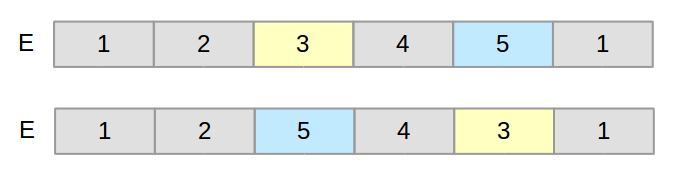
\includegraphics[width=400pt]{images/algo_05_mutation.png}
	\caption{Beispiel: Mutation eines Individuums}
	\label{fig:algo-sample-mutation}
\end{figure}

Hierbei werden per Zufall die beiden Knoten 3 und 5 ausgewählt. Deren Position in der Liste wird daraufhin einfach vertauscht, wodurch die Lösung unter Umständen völlig neue Möglichkeiten in die Population einbringt.

\subsection{Exchange}
\label{sec:exchange}

Die bisher vorgestellten Phasen beschreiben einen genetischen Algorithmus aus dem Lehrbuch, der rein single threaded funktioniert. Um diesen Algorithmus nun zu parallelisieren wird er um eine weitere Phase erweitert.\\
Die Problematik beim TSP ist, dass die Komplexität des Lösungsraumes exponentiell mit der Größe des verwendeten Graphen steigt (siehe \autoref{chap:tsp}). Um das TSP für größere Graphen mit einem genetischen Algorithmus zu lösen muss die Größe der verwendeten Population vergrößert werden, damit die Population allein durch die schiere Anzahl an Lösungsmöglichkeiten nicht genetisch verhungert. Jedoch benötigen größere Populationen deutlich mehr Rechenleistung pro Generation und so können sehr große Graphen nur langsam gelöst werden.\\
Um diese Problematik zu lösen wurde die Population auf mehrere Prozesse verteilt. Jeder dieser Prozesse ist single threaded und berechnet den genetischen Algorithmus gemäß den bereits vorgestellten Phasen vollständig unabhängig von den anderen Prozesse. Am Ende jeder Generation treten jedoch alle Prozesse in die \textit{Exchange} Phase ein. In dieser Phase senden alle Prozesse einen Anteil von 10\% ihrer Population an einen anderen Prozess. Der sendende Prozess löscht diese Individuen aus seiner Population und der empfangende Prozesse fügt die erhaltenen Individuen in seine Population ein. Hierzu müssen alle Prozesse die gleiche Populationsgröße besitzen, sodass nach dem Austausch die Population wieder gleich groß ist wie zuvor. Durch diesen Austausch von Individuen entsteht ein Austausch von Genmaterial, sodass die verschiedenen Populationen der Prozesse näherungsweise wie eine einzige große Population funktionieren. So agieren 10 Prozesse mit einer Population von 1000 Individuen so wie ein einziger Prozess mit 10000 Individuen. Darüber hinaus kann jeder Prozess die rechenintensiven Phasen auf einem separaten Kern mit einer Populationsgröße von 1000 statt 10000 ausführen, sodass die Prozessgemeinschaft abzüglich des Kommunikationsoverheads näherungsweise so schnell abläuft wie ein einzelner Prozess mit nur 1000 Individuen.\\
In \autoref{fig:algo-sample-exchange} ist zu sehen, wie der Austausch der Individuen mit fünf Prozessen funktioniert.

\begin{figure}[ht]
  	\centering
	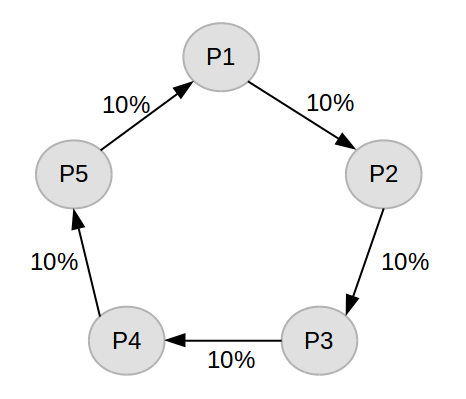
\includegraphics[width=300pt]{images/algo_06_exchange.png}
	\caption{Beispiel: Austausch der Individuen}
	\label{fig:algo-sample-exchange}
\end{figure}

Hierbei wird ein Ringaustauschverfahren verwendet. Jeder Prozess hat eine eindeutige ID und gibt seine Individuen an den jeweils nächsten Prozess  weiter, also P1 senden an P2, P2 an P3, usw. So wird ein kompliziertes Kommunikationsverfahren zur Findung von Partnerprozessen vermieden, um den Netzwerkoverhead möglichst niedrig zu halten.

\chapter{Technologie}
\label{chap:technologie}

Programmiersprache; json; build system; unit test; github; travis CI; gnuplot etc.

\section{MPI}
\label{sec:mpi}

wie funktioniert mpi prinzipiell?; p2p verbindung; ssh; broadcast, send, receive 

\chapter{Testumgebung}
\label{chap:testumgebung}

MAC pool; programmierung auf linux;

\chapter{Ergebnisse}
\label{chap:ergebnisse}

\clearpage
\pagenumbering{Roman}
\lstlistoflistings
\addcontentsline{toc}{chapter}{\lstlistlistingname}
\listoffigures
\listoftables
\bibliographystyle{plain}
\bibliography{literature}

\end{document}